\chapter{Processing Elements}
\section{Instruction Set Processor (ISP)}
\subsection{von-Neumann-/Princeton-Architektur}
\todo{Grafik}
\begin{figure}[H]
    \centering
    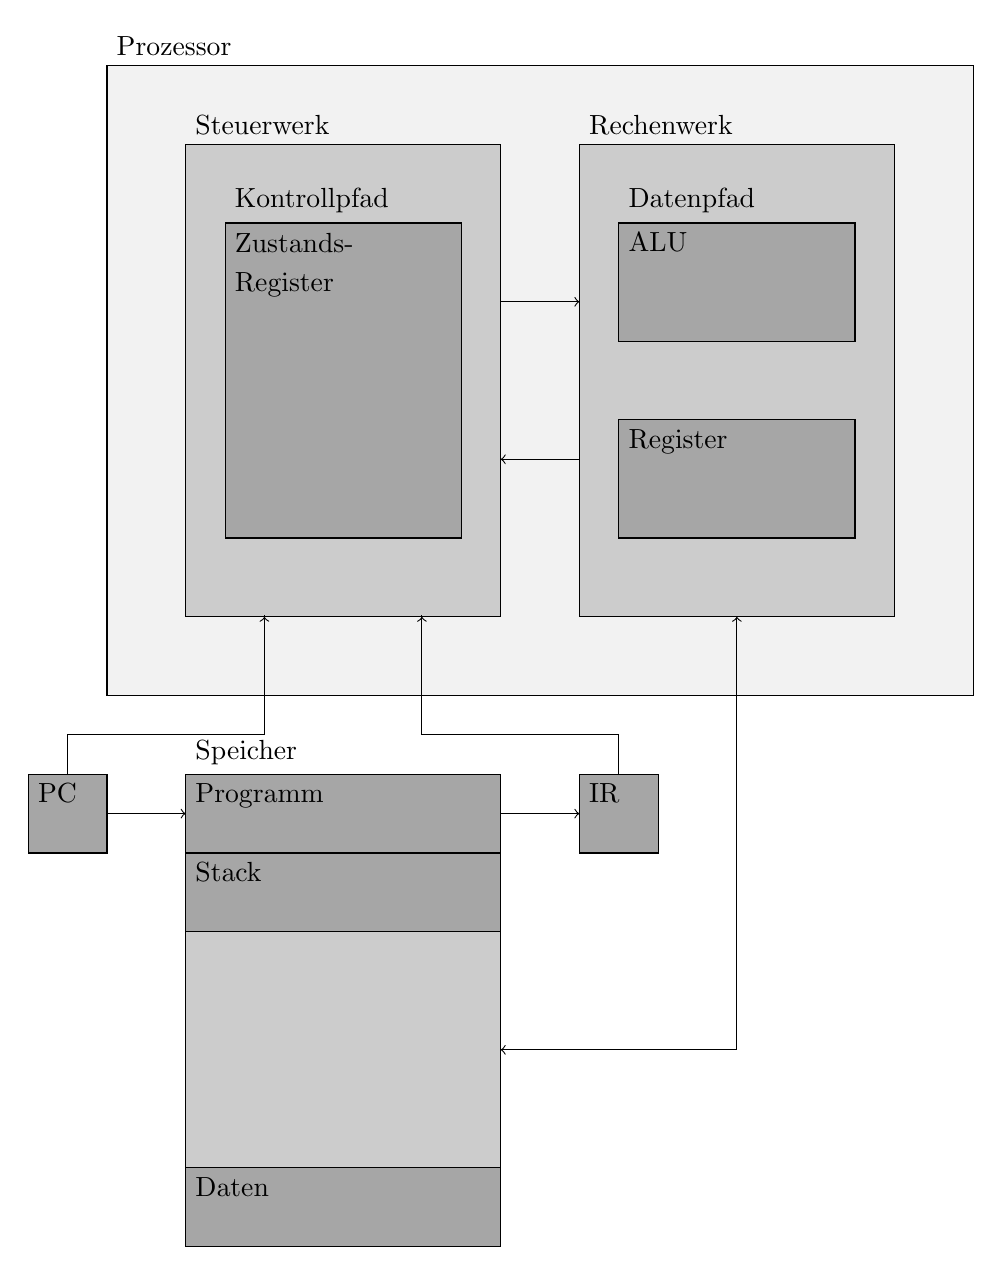
\begin{tikzpicture}
        \filldraw [draw=black,fill=gray!10] (-1,7) rectangle (10,15);
        \filldraw [draw=black,fill=gray!40] (0,0) rectangle (4,6);
        \filldraw [draw=black,fill=gray!40] (0,8) rectangle (4,14);
        \filldraw [draw=black,fill=gray!40] (5,8) rectangle (9,14);
        \filldraw [draw=black,fill=gray!70] (0.5,9) rectangle (3.5,13);
        \filldraw [draw=black,fill=gray!70] (5.5,11.5) rectangle (8.5,13);
        \filldraw [draw=black,fill=gray!70] (5.5,9) rectangle (8.5,10.5);
        \filldraw [draw=black,fill=gray!70] (5,5) rectangle (6,6);
        \filldraw [draw=black,fill=gray!70] (-2,5) rectangle (-1,6);
        \filldraw [draw=black,fill=gray!70] (0,6) rectangle (4,5);
        \filldraw [draw=black,fill=gray!70] (0,5) rectangle (4,4);
        \filldraw [draw=black,fill=gray!70] (0,0) rectangle (4,1);
        \draw (-1,15) node[above right] {Prozessor};
        \draw (0,14) node[above right] {Steuerwerk};
        \draw (5,14) node[above right] {Rechenwerk};
        \draw (0,6) node[above right] {Speicher};
        \draw (0.5,13) node[above right] {Kontrollpfad};
        \draw (0.5,13) node[below right] {Zustands-};
        \draw (0.5,12.5) node[below right] {Register};
        \draw (5.5,13) node[above right] {Datenpfad};
        \draw (5.5,13) node[below right] {ALU};
        \draw (5.5,10.5) node[below right] {Register};
        \draw (5,6) node[below right] {IR};
        \draw (-2,6) node[below right] {PC};
        \draw (0,6) node[below right] {Programm};
        \draw (0,5) node[below right] {Stack};
        \draw (0,1) node[below right] {Daten};
        \draw [->] (4,12) -- (5,12);
        \draw [->] (5,10) -- (4,10);
        \draw [->] (7,2.5) -- (4,2.5);
        \draw [->] (7,2.5) -- (7,8);
        \draw [->] (4,5.5) -- (5,5.5);
        \draw (5.5,6) |- (3,6.5);
        \draw [->] (3,6.5) |- (3,8);
        \draw [->] (-1,5.5) -- (0,5.5);
        \draw (-1.5,6) |- (1,6.5);
        \draw [->] (1,6.5) |- (1,8);
    \end{tikzpicture}
    \caption{Aufbau eines von-Neumann Prozessors}
\end{figure}
\subsection{Befehlszyklus}
\begin{enumerate}
    \item Befehl holen (fetch)
    \item Befehl dekodieren (decode)
    \item Operanden holen (load)
    \item Befehl ausführen (execute)
    \item Daten speichern (write back)
\end{enumerate}

\begin{table}[H]
    \centering
    \begin{tabular}{p{.5\textwidth}p{.5\textwidth}}
        \toprule
        Pro & Contra \\
        \midrule
        Analyse einfach & Auslastung gering \\
        Speicher flexibel benutzbar & von-Neumann Flaschenhals (Daten und Befehle über den selben Bus)\\
        \bottomrule
    \end{tabular}
\end{table}

\subsection{Harvard-Architektur}
\begin{figure}[H]
    \centering
    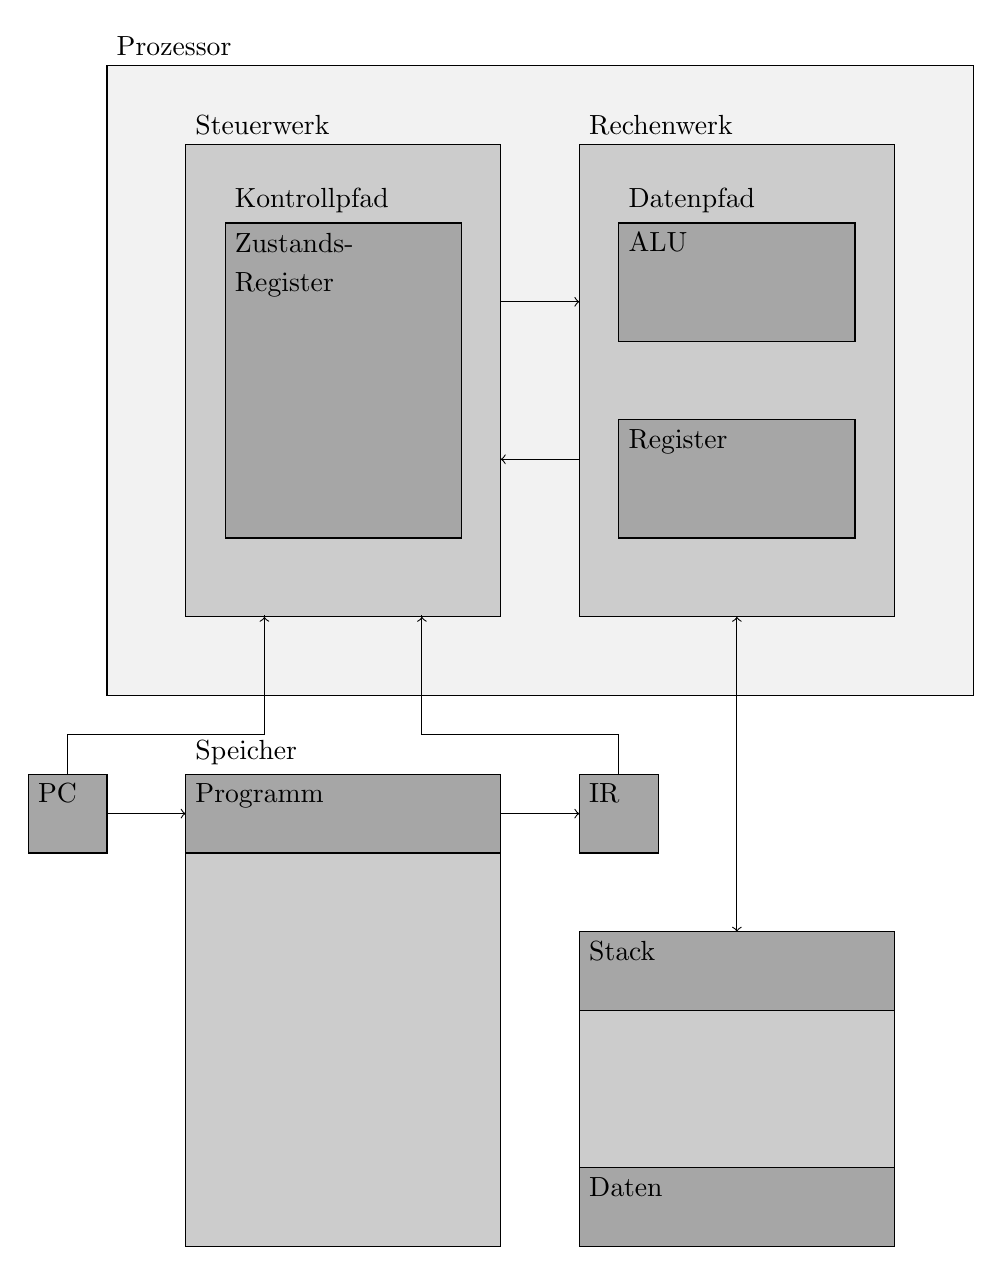
\begin{tikzpicture}
        \filldraw [draw=black,fill=gray!10] (-1,7) rectangle (10,15);
        \filldraw [draw=black,fill=gray!40] (0,0) rectangle (4,6);
        \filldraw [draw=black,fill=gray!40] (0,8) rectangle (4,14);
        \filldraw [draw=black,fill=gray!40] (5,8) rectangle (9,14);
        \filldraw [draw=black,fill=gray!40] (5,0) rectangle (9,4);
        \filldraw [draw=black,fill=gray!70] (0.5,9) rectangle (3.5,13);
        \filldraw [draw=black,fill=gray!70] (5.5,11.5) rectangle (8.5,13);
        \filldraw [draw=black,fill=gray!70] (5.5,9) rectangle (8.5,10.5);
        \filldraw [draw=black,fill=gray!70] (5,5) rectangle (6,6);
        \filldraw [draw=black,fill=gray!70] (-2,5) rectangle (-1,6);
        \filldraw [draw=black,fill=gray!70] (0,6) rectangle (4,5);
        \filldraw [draw=black,fill=gray!70] (5,4) rectangle (9,3);
        \filldraw [draw=black,fill=gray!70] (5,0) rectangle (9,1);
        \draw (-1,15) node[above right] {Prozessor};
        \draw (0,14) node[above right] {Steuerwerk};
        \draw (5,14) node[above right] {Rechenwerk};
        \draw (0,6) node[above right] {Speicher};
        \draw (0.5,13) node[above right] {Kontrollpfad};
        \draw (0.5,13) node[below right] {Zustands-};
        \draw (0.5,12.5) node[below right] {Register};
        \draw (5.5,13) node[above right] {Datenpfad};
        \draw (5.5,13) node[below right] {ALU};
        \draw (5.5,10.5) node[below right] {Register};
        \draw (5,6) node[below right] {IR};
        \draw (-2,6) node[below right] {PC};
        \draw (0,6) node[below right] {Programm};
        \draw (5,4) node[below right] {Stack};
        \draw (5,1) node[below right] {Daten};
        \draw [->] (4,12) -- (5,12);
        \draw [->] (5,10) -- (4,10);
        \draw [<->] (7,4) -- (7,8);
        \draw [->] (4,5.5) -- (5,5.5);
        \draw (5.5,6) |- (3,6.5);
        \draw [->] (3,6.5) |- (3,8);
        \draw [->] (-1,5.5) -- (0,5.5);
        \draw (-1.5,6) |- (1,6.5);
        \draw [->] (1,6.5) |- (1,8);
    \end{tikzpicture}
    \caption{Aufbau eines Harvard Prozessors}
\end{figure}
\begin{table}[H]
    \centering
    \begin{tabular}{p{.5\textwidth}p{.5\textwidth}}
        \toprule
        Pro & Contra \\
        \midrule
        Auslastung & Fragmentierter Speicher \\
        Kein Flaschenhals & Analyse schwierig \\
        Schnellere Abarbeitung & Schwierig bei Datenabhängigkeiten \\
        \bottomrule
    \end{tabular}
\end{table}

\section{Application Specific Instruction Set Processor (ASIP)}
Regulärer ISP wird durch zusätzliche Instruktionen (und damit auch Hardware) für ein bestimmtes Einsatzgebiet optimiert, 
z.B. durch zusätzlich \glqq{}Multiply-Accumulate\grqq{}-Einheit oder auch komplette FFT-Operationen.
Beispiel: DSP (Digital Signal Processpr).
\begin{figure}[H]
    \centering
    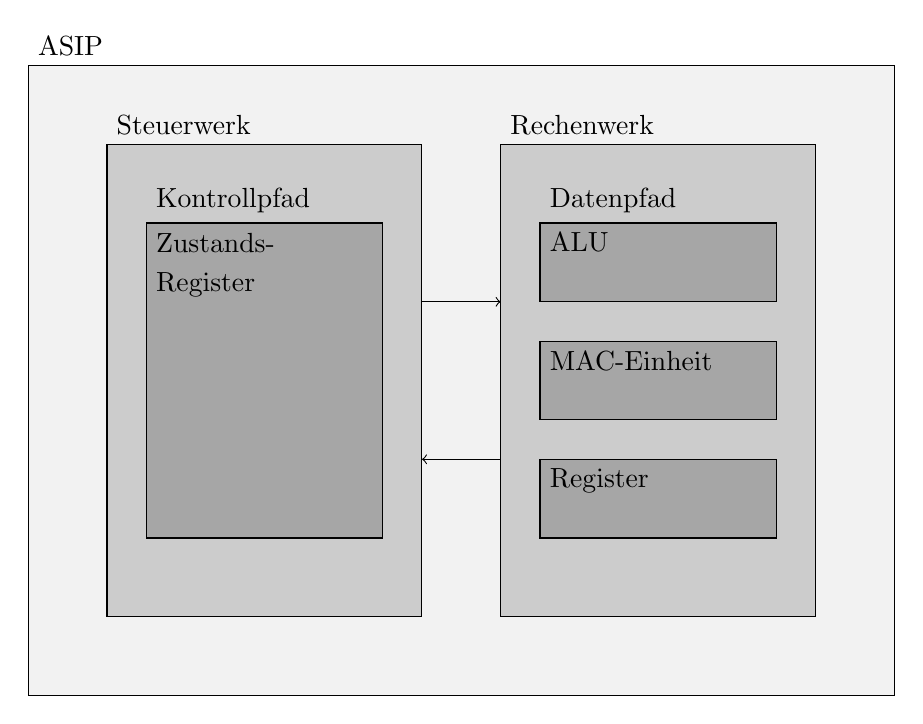
\begin{tikzpicture}
        \filldraw [draw=black,fill=gray!10] (-1,7) rectangle (10,15);
        \filldraw [draw=black,fill=gray!40] (0,8) rectangle (4,14);
        \filldraw [draw=black,fill=gray!40] (5,8) rectangle (9,14);
        \filldraw [draw=black,fill=gray!70] (0.5,9) rectangle (3.5,13);
        \filldraw [draw=black,fill=gray!70] (5.5,12) rectangle (8.5,13);
        \filldraw [draw=black,fill=gray!70] (5.5,10.5) rectangle (8.5,11.5);
        \filldraw [draw=black,fill=gray!70] (5.5,9) rectangle (8.5,10);
        \draw (-1,15) node[above right] {ASIP};
        \draw (0,14) node[above right] {Steuerwerk};
        \draw (5,14) node[above right] {Rechenwerk};
        \draw (0.5,13) node[above right] {Kontrollpfad};
        \draw (0.5,13) node[below right] {Zustands-};
        \draw (0.5,12.5) node[below right] {Register};
        \draw (5.5,13) node[above right] {Datenpfad};
        \draw (5.5,13) node[below right] {ALU};
        \draw (5.5,11.5) node[below right] {MAC-Einheit};
        \draw (5.5,10) node[below right] {Register};
        \draw [->] (4,12) -- (5,12);
        \draw [->] (5,10) -- (4,10);
    \end{tikzpicture}
    \caption{Aufbau eines ASIP mit zusätzlicher MAC-Einheit}
\end{figure}

\section{Application Specific Processor}
Nicht mehr programmierbar, Prozessor kann nur wenige vorkonfigurierte Befehle ausführen, Steuerung erfolgt über eine spezielle Logik, oftmals in Form einer
State-Machine.
\begin{figure}[H]
    \centering
    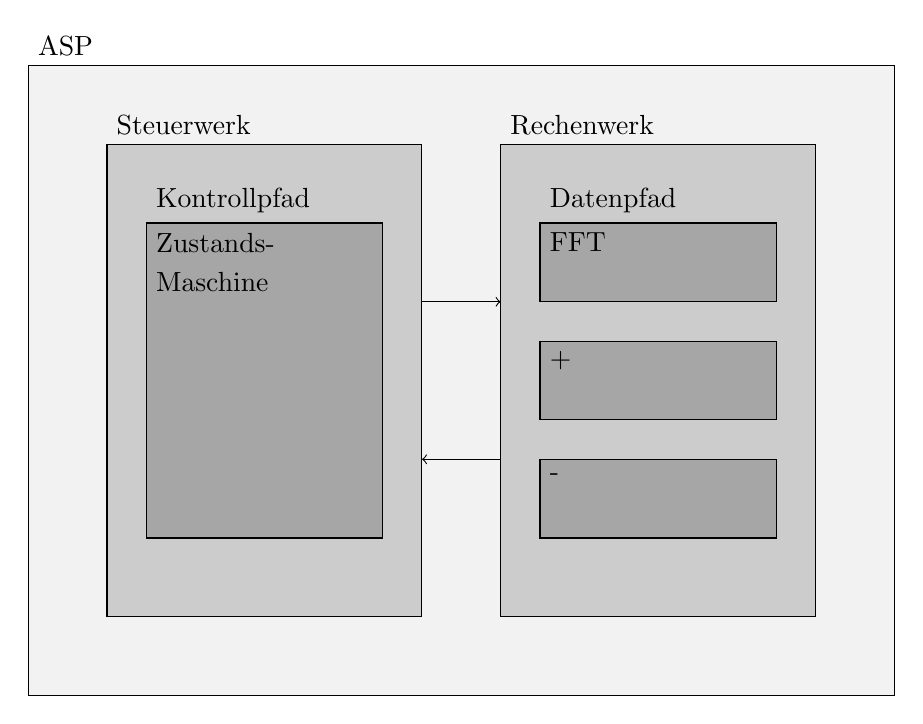
\begin{tikzpicture}
        \filldraw [draw=black,fill=gray!10] (-1,7) rectangle (10,15);
        \filldraw [draw=black,fill=gray!40] (0,8) rectangle (4,14);
        \filldraw [draw=black,fill=gray!40] (5,8) rectangle (9,14);
        \filldraw [draw=black,fill=gray!70] (0.5,9) rectangle (3.5,13);
        \filldraw [draw=black,fill=gray!70] (5.5,12) rectangle (8.5,13);
        \filldraw [draw=black,fill=gray!70] (5.5,10.5) rectangle (8.5,11.5);
        \filldraw [draw=black,fill=gray!70] (5.5,9) rectangle (8.5,10);
        \draw (-1,15) node[above right] {ASP};
        \draw (0,14) node[above right] {Steuerwerk};
        \draw (5,14) node[above right] {Rechenwerk};
        \draw (0.5,13) node[above right] {Kontrollpfad};
        \draw (0.5,13) node[below right] {Zustands-};
        \draw (0.5,12.5) node[below right] {Maschine};
        \draw (5.5,13) node[above right] {Datenpfad};
        \draw (5.5,13) node[below right] {FFT};
        \draw (5.5,11.5) node[below right] {+};
        \draw (5.5,10) node[below right] {-};
        \draw [->] (4,12) -- (5,12);
        \draw [->] (5,10) -- (4,10);
    \end{tikzpicture}
    \caption{Aufbau eines ASP, der nur FFT,+ und - Operationen durchführt}
\end{figure}

\section{Beispiel: Aufbau eines Schnurlosen DECT-Telefons}
\todo{Grafik}
Oftmals wird ein ISP mit zugehöriger RF-Hardware auf einem Chip-Integriert (z.B. in Mobiltelefonen), dann spricht man von einem Sytem-on-a-Chip (SoC).

\section{Wie kommunizieren PEs in heterogenen Systemen?}
\subsection{Gemeinsame Ressourcen (Speicherkopplung)}
\todo{Grafik}
Alle PEs können über einen Bus auf eine gemeinsame Ressource (für gewöhnlich Speicher) zugreifen. 
Für die Synchronisation ist ein \glqq{}Arbiter\grqq{} (Richter) sowie ein Bus-Controller in jedem PE notwendig.

\subsection{Direkte Verbindung}
Direkte Verbindung zwischen allen PEs die kommunizieren müssen, Arbitrierung ist nicht notwendig, mehrere PEs können gleichzeitig kommunizieren. 
Es ist wieder ein Controller für jede Verbindung von nöten, zudem muss dieser eventuell Daten puffern. 
Bei $n$ PEs sind im Worstcase $\frac{(n-1)\cdot n}{2} \in  \mathcal{O}(n^2)$ Verbindung notwendig.

\subsection{Tiled-Architecture}
Bei einer Tiled-Architecture oder Network-on-a-Chip (NOC) werden jeweils wenige PEs über eine gemeinsame Resource verbunden. 
Diese Gruppen an PEs werden dann über ein Gitter aus Leitungen verbunden.
\todo{Grafik}
